%!TEX root = ../main.tex
\section{Connectivity Pattern}
\captionsetup[subfigure]{justification=raggedright, singlelinecheck=off}
\begin{figure}
    \centering
    \begin{subfigure}[b]{0.98 \linewidth}
    \centering
    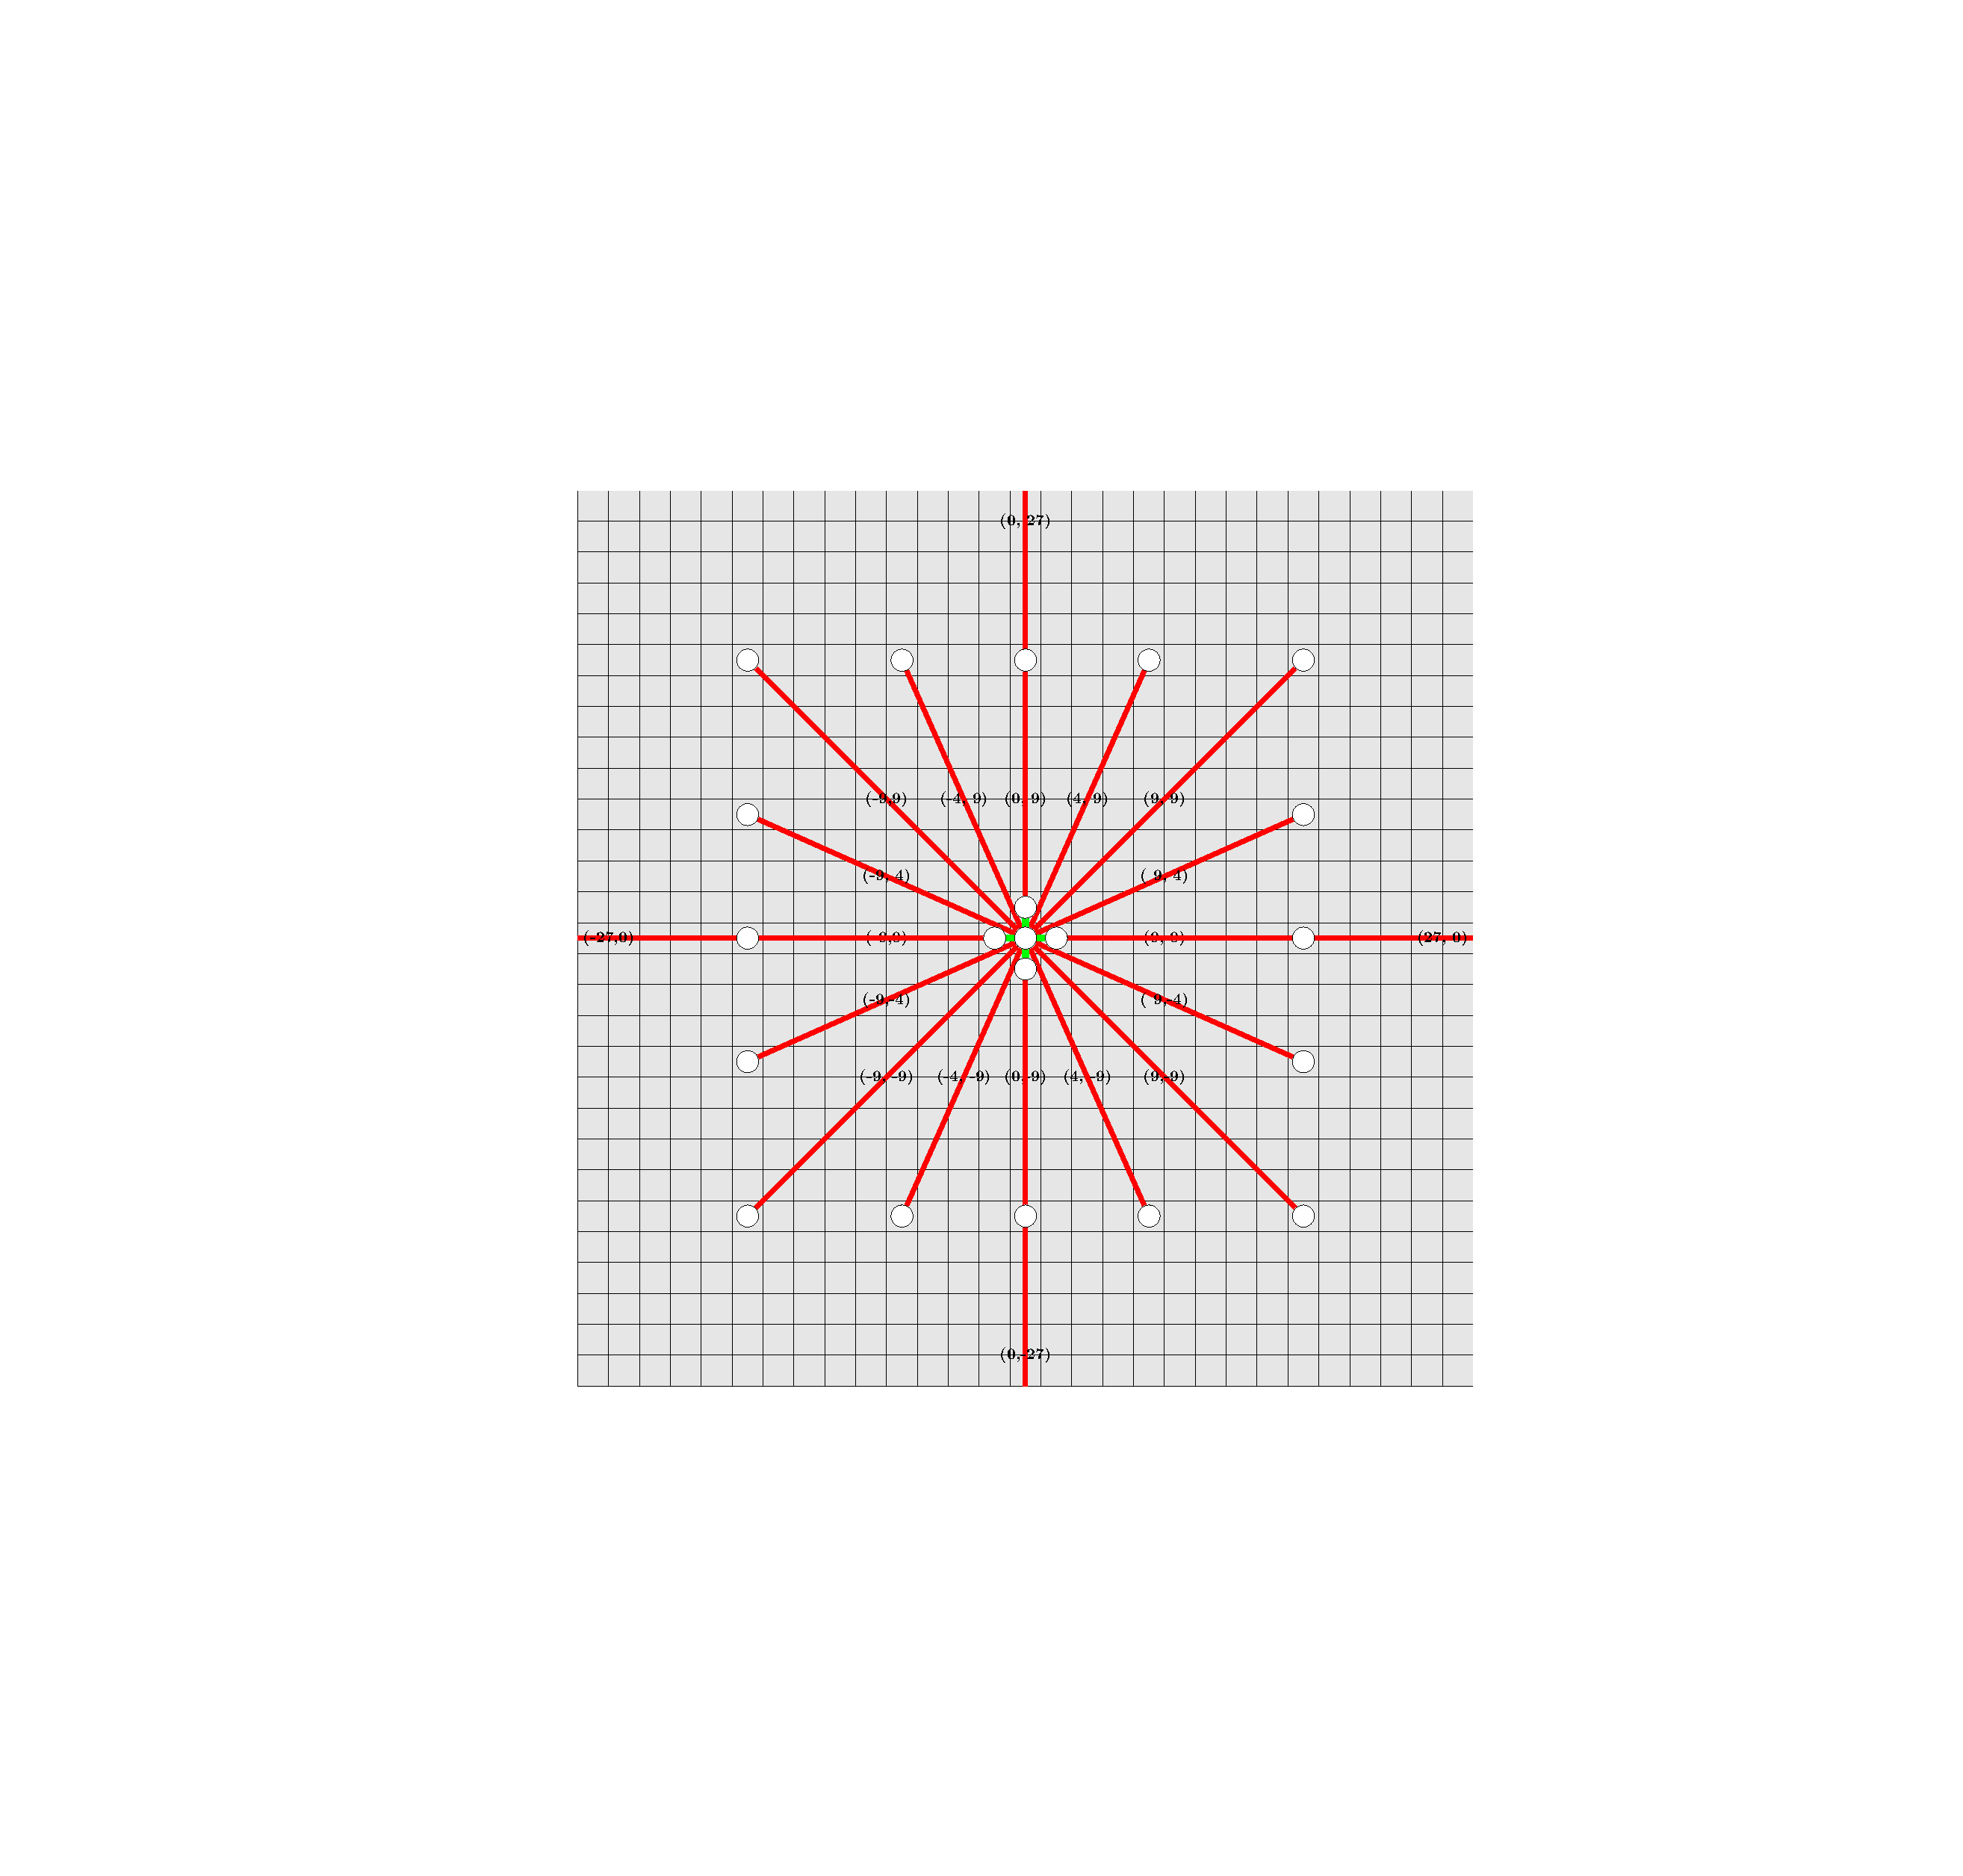
\includegraphics[width=0.8\linewidth,valign=t]{images/2d_connection.pdf}%
    \caption{XY-plane neighborhood with local attractive edges,
     a sparse repulsive edges with approximate radius 9 and further long-range connections with distance 27}\label{fig:2d-connection}
    \end{subfigure}\hfill

    \begin{subfigure}[b]{0.98 \linewidth}
    \centering
    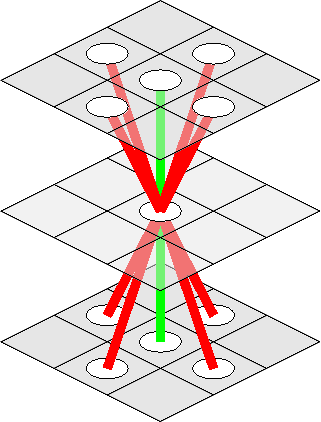
\includegraphics[width=0.6\linewidth, valign=t]{images/3d_connection3.pdf}
    \caption{Due to the high anisotropy of the data we limit the Z-plane edges to a distance of 1. The direct neighbors are attractive, whereas the indirect neighbors are repulsive.}\label{fig:3d-connection}
    \end{subfigure}%
    \caption{Local neighborhood structure of attractive~(green) and repulsive~(red) edges in the mutex watershed graph.}
    \label{fig:connectivity}
\end{figure}

Ideally we would like to use a fully connected graph of repulsive edges to model every possible pairwise exclusion constraint. However, since we use a neural network we can only predict the edge weights of a limited number of edges which limits us to a sparse and regular connectivity pattern.

We picked a sparse ring of in-plane repulsive edges and additional longer-range in-plane edges which were necessary to split regions reliably (see Figure \ref{fig:2d-connection}).
We also added connections to the indirect neighbors in the lower adjacent slice to ensure correct 3D connectivity (see Figure \ref{fig:3d-connection}). In our experiments, we pick a subset of repulsive edges, by using strides of 2 in the XY-plane in order to avoid artifacts caused by occasional very thick membranes. Note that the stride is not applied to local (attractive) edges, but only to long-range (repulsive) edges. 
%This reduces artifacts in form of single pixel segments due to thick boundaries.
%It also decrease the runtime of the mutex watershed by reducing the total number of edges considered by Algorithm \ref{algo_code}.

In total, $C^+$ attractive and $C^-$ repulsive edges are defined for each pixel, resulting in $C^+ + C^-$ output channels in the network. 
We partition the set of attractive / repulsive edges into subsets $H^+$ and $H^-$ that contain all edges at a specific offset, attractive edges:
$\label{edgesets}
    E^+ = {\bigcup_{c}^{C^+}} H^+_{c}$ and repulsive edges analogously. 
Each element of the subsets $H^+_{c}$ and $H^-_{c}$ corresponds to a specific channel predicted by the network. We further assume that weights take values in $[0,1]$ and adopt the same conventions for attraciveness / repulsion as in section \ref{3_methods}. 

\subsubsection*{Network architecture and training}
We use the 3D U-Net \cite{ronneberger_15_u-net,cciccek20163d} architecture, as proposed in \cite{funke2017deep}. %It is illustrated in Figure \ref{fig:architecture}.

Our training targets for attractive / repulsive edges $\hat w^\pm$ can be derived from a ground truth label image $\hat L$ according to
\begin{equation}
    \hat w^+_e = \begin{cases}
        1 , &\text{ if } \hat L_i = \hat L_j \textrm{with} \, e = e_{ij} \\
        0 , & \text{otherwise}
    \end{cases}\quad
\end{equation}
\begin{equation}
    \hat w^-_e = \begin{cases}
        0 , &\text{ if } \hat L_i = \hat L_j  \textrm{with} \, e = e_{ij} \\
        1 , & \text{otherwise}
    \end{cases}
\end{equation}

Here, $i$ and $j$ are the indices of image pixels and $e_{ij}$ denotes the edge connecting them.
Next, we define the loss terms

\begin{equation} \label{dice_plus}
    \mathcal{J}^+_{c} = - \frac{\sum_{e \in H^+_{c}} (1 - w^+_e) (1 - \hat w^+_e)}{\sum_{e \in H^+_{c}} ((1 - w^+_e)^2 + (1 -\hat w^+_e)^2)} 
\end{equation}
\begin{equation}
\mathcal{J}^-_{c} = - \frac{\sum_{e \in H^-_{c}} w^-_e {\hat w^-}_e}{\sum_{e \in H^-_{c}} ((w^-_e)^2 + (\hat w^-_e)^2)}
\end{equation}
for attractive edges (i. e. channels) and repulsive edges (i. e. channels).

Equation \ref{dice_plus} is the S{\o}rensen-Dice coefficient \cite{dice1945measures,sorensen1948method} formulated for fuzzy set membership values and a product T-norm.
During training we minimize the sum of attractive and repulsive loss terms $\mathcal{J} = \sum_{c}^{C^+} \mathcal{J}^{+}_{c} + \sum_{c}^{C^-} \mathcal{J}^{-}_{c}$. This corresponds to summing up the channel-wise S{\o}rensen-Dice loss. 
The terms of this loss are robust against prediction and/or target sparsity, a desirable quality for neuron segmentation: since membranes are very thin, they occupy very few pixels in the volume. 
More precisely, if $w^{+}_e$ or $\hat w^{+}_e$ (or both) are sparse, we can expect the denominator $\sum_e(({w^{+}_e})^2 + ({\hat {w}}^+_e)^2)$ to be small,
which has the effect that the numerator is adaptively weighted higher. 
In this sense, the S{\o}rensen-Dice loss at every pixel $i$ is conditioned on the global image statistics, which is not the case for a Hamming-distance based loss like Binary Cross-Entropy or Mean Squared Error. 

We optimize this loss using the Adam optimizer and additionally condition learning rate decay on 
the Adapted Rand Score \cite{isbi2012challenge} computed on the training set every 100 iterations.
During training, we augment the data set by performing in-plane rotations by multiples of 90 degrees, flips along the x- and y- axis as well as elastic deformations.
At prediction time, we use test time data augmentation, presenting the network with
seven different versions of the input obtained by a combination of rotations by a multiple of 90 degrees, axis-aligned flips and transpositions.
The network predictions are then inverse-transformed to correspond to the original image, and the results averaged.
